% Description: Draw Graphics

% Note
% 1. Tikz package can be used to draw graphics from within the LaTeX document.
% 2. Drawing a picture should be programmed.
% 3. Extensive documentation is available for the Tikz package.
% 4. Many examples can be found on the internet.
% 5. Extensions available to easy creation of diagrams, flowcharts and so forth.

\documentclass{article}

\usepackage{tikz}

\begin{document}

\begin{figure}[h!]
    \begin{center}
        % Embed our tikzpicture in a figure environment.
        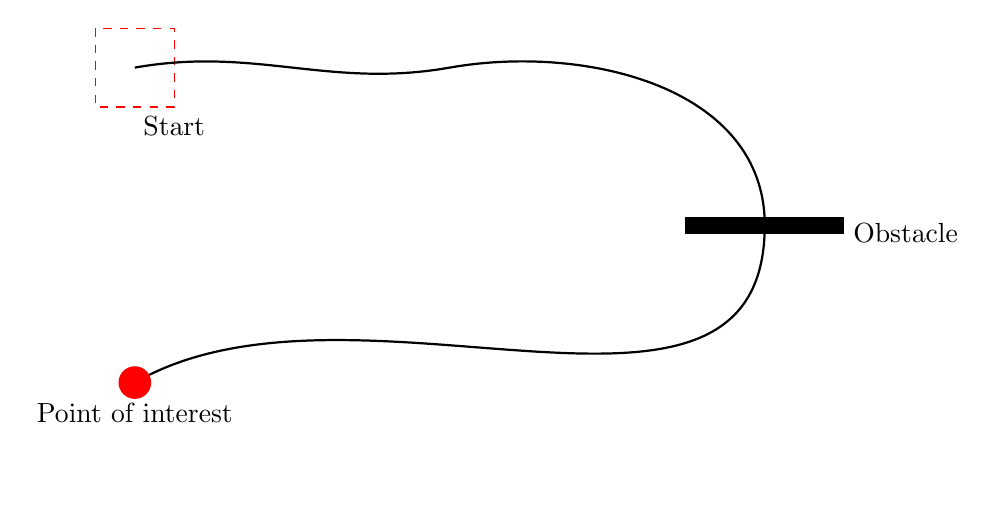
\begin{tikzpicture}
            % Specifies the rectangle should be red and dashed, no magic here.
            % Location of the rectangle (-2.5,2.5) in cartesian coordinates.
            % Set the size of the rectangle (-1.5,1.5).
            % Text is usually placed as a so-called node (text-node) in our picture.
            % Define the text to have black color and set the position to below our rectangle.
            \draw [red,dashed] (-2.5,2.5) rectangle (-1.5,1.5) node [black,below] {Start};          % Draws a rectangle
            % Draw a line by specifying a path in Tikz
            \draw [thick] (-2,2)                                                                    % Draws a line
            % The to command is used to specify a point of the path.
            % Tikz usually draws straight lines between the points. The bent lines can be accomplished by setting the in
            % and out angle in brackets.
            to [out=10,in=190] (2,2)
            to [out=10,in=90] (6,0)
            % Terminate each command with a semicolon inside of the tikzpicture environment.
            to [out=-90,in=30] (-2,-2);
            \draw [fill] (5,0.1) rectangle (7,-0.1) node [black,right] {Obstacle};                  % Draws a rectangle
            \draw [red,fill] (-2,-2) circle [radius=0.2] node [black,below=4] {Point of interest};  % Draws a circle
        \end{tikzpicture}
        \caption{Example graphic made with tikz.}
    \end{center}
\end{figure}

\end{document}